\begin{frame}{Architecture: High Level}
  \begin{columns}
      \begin{column}{8.5cm}
      \begin{itemize}
        \item \textit{Inspiration:} KART
        $$f(x_1,\dots,x_n) = \sum_{q=0}^{2n}\phi_q\left(\sum_{p=1}^n\psi_{q,p}(x_p)\right)$$
        \item We just need to learn the univariate functions $\psi$ and $\phi$ and perform addition
        \vspace{0.5em}
        \item \strong{($\rightarrow$)} A shallow KAN representing the above equation, with $n=2$ input variables $x_p$,\\ $2n+1=5$ $\phi_{\text{s}}$ and  $f(x_1,x_2)$ as the output
        \vspace{0.5em}
        \item Learnable activation functions are positioned on edges and summation is performed on nodes
      \end{itemize}
    \end{column}

    \begin{column}{5cm}
      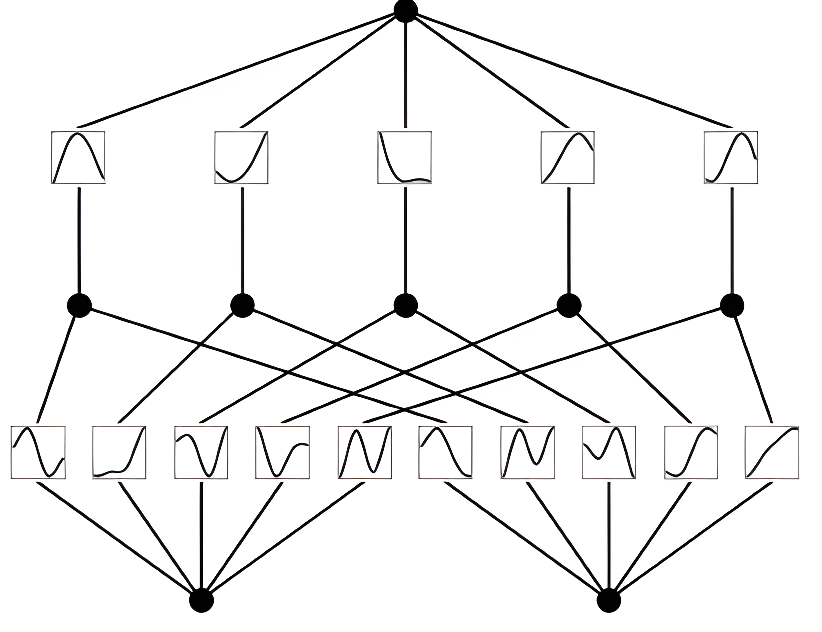
\includegraphics[width=5cm]{contents/images/KAN_arch_simple}
    \end{column}
  \end{columns}
\end{frame}

\begin{frame}{Architecture: Comparison with MLP}
    \strong{Shallow Formula} \vspace{0.3em}
    \begin{itemize}
        \item Though KART ensures exact representation and UAT guarantees approximation, relaxing KART's assumptions positions both as function approximators \vspace{0.5em}
        \item UAT lacks guarantees on shallow MLP size, and KART provides no method to compute the relative functions \vspace{0.5em}
        %A set G\subseteq F of functions is called dense in a function space F, if it can approximate any function f\in F to an arbitrary degree of accuracy.
        %In other words, given any real function f\in F and ε>0, there is a real function g\in G for which |g(x) - f(x)|<ε
        \item MLP uses fixed activations on nodes and learnable weights on edges, while KAN employs fixed learnable functions on edges and summation on nodes \vspace{0.5em}
    \end{itemize}
\end{frame}

\begin{frame}{Architecture: Comparison with MLP}
    \strong{Deep Formula} \vspace{0.3em}
    \begin{itemize}
        \item Shifting to deep formula to avoid UAT's and KART's restrictions \vspace{0.3em}
        \item KAN shifts non-linearity computation to the composition of $\phi_{\text{s}}$ rather than the
        weights and activation functions in MLPs \vspace{0.3em}
        \item KAN defines a \textit{KAN layer} with $n_{\text{in}}$-D inputs and $n_{\text{out}}$-D
        outputs as a matrix of 1D functions, stacking these layers (note how we are drifting further away from KART)\vspace{0.3em}
        \item So, the dimensions of the KAN are \textit{not} restricted to $[n, 2n+1, 1]$
    \end{itemize}
\end{frame}

\begin{frame}{Architecture: Lower Level}
    \begin{itemize}
        \item The learnable univariate functions are parametrized as a \textbf{B-spline (basis spline) curves} with learnable coefficients of local B-splines \vspace{0.3em}
        \item Splines are a transformation that maps control points to a smooth curve, aiming to generally follow the shape of these points \vspace{0.3em}
        \item Let us present the B-splines in depth \vspace{0.3em}
    \end{itemize}
\end{frame}

\begin{frame}{B\'ezier curves: Linear}
        To create a path between 2 points $P_0$ and $P_1$, we perform \textbf{linear interpolation} :
         \vspace{1em}
        $$P(t) = (1-t)P_0 + tP_1$$
        \vspace{0.5em}
        \begin{center}
            
\includegraphics[width=5cm]{contents/images/linear_interpolation_1}
        \end{center}
\end{frame}

\begin{frame}{B\'ezier curves: Quadratic}
    \begin{itemize}
        \item If we add a third point $P_2$, then we have two lines connecting them and we can perform linear interpolation to them as well
        \vspace{1em}
        \begin{center}
            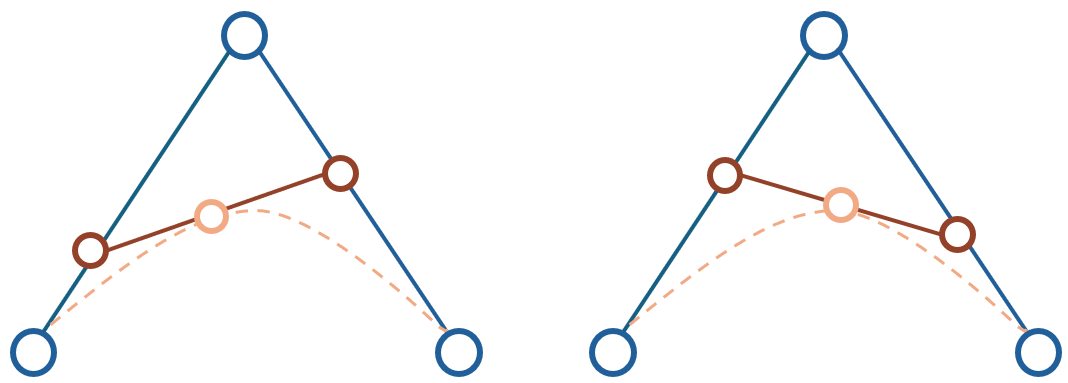
\includegraphics[width=10cm]{contents/images/quadratic_bezier_3}
        \end{center}\vspace{1em}
        \item This curve is called a \textbf{quadratic} \strong{B\'ezier curve}
    \end{itemize}
\end{frame}

\begin{frame}{B\'ezier curves: Cubic and higher}
    \begin{itemize}
        \item In the same spirit, we can define the \textbf{cubic B\'ezier curve} (and any other degree, respectively)
        \vspace{1em}
        \begin{center}
            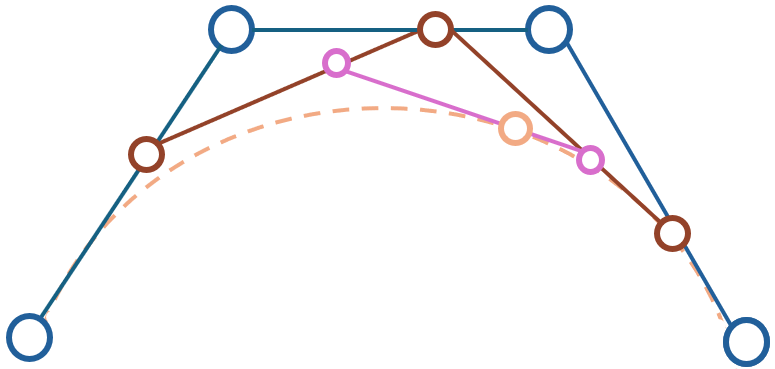
\includegraphics[width=6cm]{contents/images/cubic_bezier}
        \end{center} \vspace{0.8em}
        \item We call the points \textbf{control points}, since the control the curvature
    \end{itemize}
\end{frame}

\begin{frame}{B\'ezier curves: Algorithms}
    \begin{itemize}
        \item This repeated linear interpolation is called the \textbf{de Casteljau} algorithm \vspace{0.2em}
        \item A less expensive method for computing B\'ezier curves involves solving the \textbf{Bernstein polynomials} which are the linear interpolation equations expressed wrt the points
    \end{itemize}
    \begin{columns}
            \begin{column}{5cm}
                 \begin{center}
                    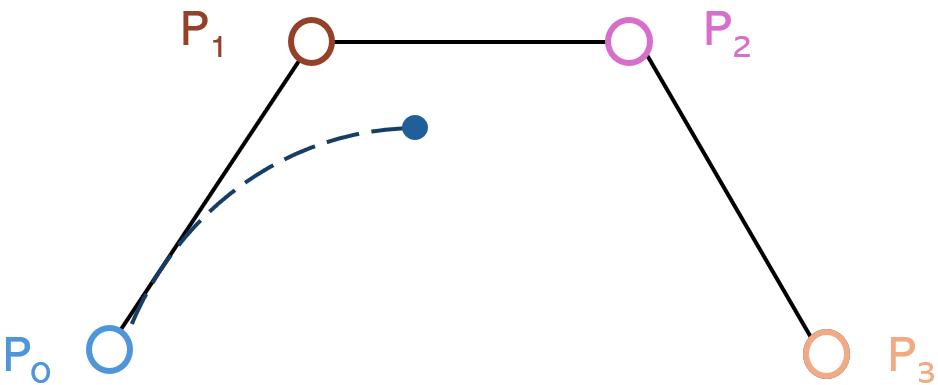
\includegraphics[width=5cm]{contents/images/cubic_bernstein}
                \end{center}
            \end{column}
            \begin{column}{2.5cm}
                \begin{center}
                 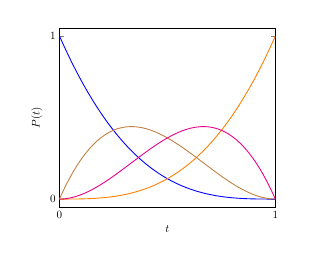
\begin{tikzpicture}[scale=0.4]
                    \begin{axis}[
                        xlabel={$t$},
                        ylabel={$P(t)$},
                        xmin=0, xmax=1,
                        ymin=-0.05, ymax=1.05,
                        xtick={0,1},
                        ytick={0,1},
                        xtick pos=both,
                        ytick pos=both,
                        grid=none,
                        %legend style={at={(1.05,1)},anchor=north west},
                        %legend cell align={left}
                    ]
                        \addplot[domain=0:1, samples=100, thick, color=blue]
                            {-x^3 + 3*x^2 - 3*x + 1};
                        %\addlegendentry{$-t^3 + 3t^2 - 3t + 1$}

                        \addplot[domain=0:1, samples=100, thick, color=orange]
                            {x^3};
                        %\addlegendentry{$t^3$}

                        \addplot[domain=0:1, samples=100, thick, color=brown]
                            {3*x^3 - 6*x^2 + 3*x};
                        %\addlegendentry{$3t^3 - 6t^2 + 3t$}

                        \addplot[domain=0:1, samples=100, thick, color=magenta]
                            {-3*x^3 + 3*x^2};
                        %\addlegendentry{$-3t^3 + 3t^2$}
                    \end{axis}
                \end{tikzpicture}
                \end{center}
            \end{column}
            \begin{column}{4.5cm}
              \scalebox{0.8}{%
                $\begin{aligned}
                  P(t) = \quad
                  & \textcolor{blue!90!black}{P_0} \cdot (-t^3 + 3t^2 - 3t + 1) +\\
                  & \textcolor{brown!70!black}{P_1} \cdot (3t^3 - 6t^2 + 3t) +\\
                  & \textcolor{magenta!80!black}{P_2}\cdot (-3t^3 + 3t^2) +\\
                  & \textcolor{orange!80!black}{P_3} \cdot (t^3)
                \end{aligned}$
              }
            \end{column}
    \end{columns}
    \begin{itemize}
        \vspace{0.2em}
        \item If we plot the factors of these polynomials we get a visualization of the influences of the control points (cf. right Illustration)
    \end{itemize}
\end{frame}

\begin{frame}{B\'ezier curves: (lack of) local control}
    \begin{itemize}
        \item One main downside of B\'ezier curves is the lack of local control
        \item This means that by changing \textbf{only one} control point, the curve can change drastically
        \item \strong{Pay attention because we will need this later on!}
    \end{itemize}
    \begin{columns}
        \begin{column}{5cm}
            \begin{figure}[h!]
                \centering
                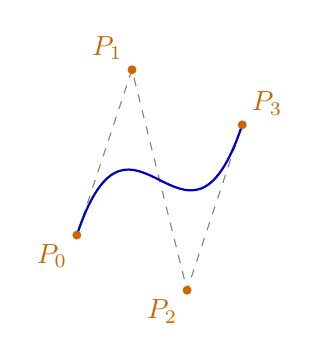
\begin{tikzpicture}[scale=0.7]
                    \coordinate (P0) at (0, 0);
                    \coordinate (P1) at (1, 3);
                    \coordinate (P2) at (2, -1);
                    \coordinate (P3) at (3, 2);

                    \draw[gray, dashed] (P0) -- (P1) -- (P2) -- (P3);
                    \draw[thick, blue!80!black] (P0) .. controls (P1) and (P2) .. (P3);

                    \filldraw[orange!80!black] (P0) circle (2pt) node[below left] {$P_0$};
                    \filldraw[orange!80!black] (P1) circle (2pt) node[above left] {$P_1$};
                    \filldraw[orange!80!black] (P2) circle (2pt) node[below left] {$P_2$};
                    \filldraw[orange!80!black] (P3) circle (2pt) node[above right] {$P_3$};
                \end{tikzpicture}
            \end{figure}
        \end{column}

        \begin{column}{5cm}
             \begin{figure}[h!]
                \centering
                 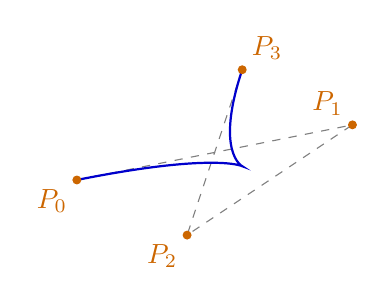
\begin{tikzpicture}[scale=0.7]
                    \coordinate (P0) at (0, 0);
                    \coordinate (P1) at (5, 1);
                    \coordinate (P2) at (2, -1);
                    \coordinate (P3) at (3, 2);

                    \draw[gray, dashed] (P0) -- (P1) -- (P2) -- (P3);

                    \draw[thick, blue!80!black] (P0) .. controls (P1) and (P2) .. (P3);

                    \filldraw[orange!80!black] (P0) circle (2pt) node[below left] {$P_0$};
                    \filldraw[orange!80!black] (P1) circle (2pt) node[above left] {$P_1$};
                    \filldraw[orange!80!black] (P2) circle (2pt) node[below left] {$P_2$};
                    \filldraw[orange!80!black] (P3) circle (2pt) node[above right] {$P_3$};
                 \end{tikzpicture}
             \end{figure}
        \end{column}
    \end{columns}
\end{frame}

\begin{frame}{B\'ezier splines}
     \begin{itemize}
        \item How to obtain local control? \textbf{Concatenate B\'ezier curves} $\rightarrow$ \strong{B\'ezier splines}
        \begin{columns}
        \begin{column}{5.5cm}
            \begin{figure}[h!]
                \centering
                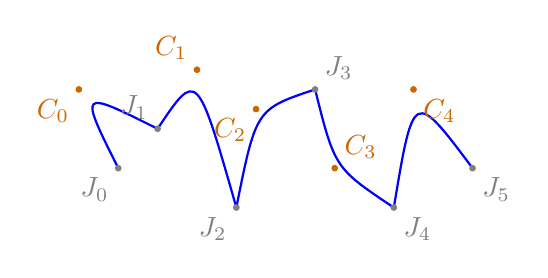
\begin{tikzpicture}[scale=0.5]
                    \coordinate (P0) at (0, 0);
                    \coordinate (P1) at (1, 1);
                    \coordinate (P2) at (3, -1);
                    \coordinate (P3) at (5, 2);
                    \coordinate (P4) at (7, -1);
                    \coordinate (P5) at (9, 0);

                    \coordinate (C0) at (-1, 2);
                    \coordinate (C1) at (2, 2.5);
                    \coordinate (C2) at (3.5, 1.5);
                    \coordinate (C3) at (5.5, 0);
                    \coordinate (C4) at (7.5, 2);

                    %\draw[gray, dashed] (P0) -- (P1) -- (P2) -- (P3) -- (P4) -- (P5);

                    \draw[thick, blue]   (P0) .. controls (C0) .. (P1);
                    \draw[thick, blue]   (P1) .. controls (C1) .. (P2);
                    \draw[thick, blue]   (P2) .. controls (C2) .. (P3);
                    \draw[thick, blue]   (P3) .. controls (C3) .. (P4);
                    \draw[thick, blue]   (P4) .. controls (C4) .. (P5);

                    \filldraw[white!50!black] (P0) circle (2pt) node[below left] {$J_0$};
                    \filldraw[white!50!black] (P1) circle (2pt) node[above left] {$J_1$};
                    \filldraw[white!50!black] (P2) circle (2pt) node[below left] {$J_2$};
                    \filldraw[white!50!black] (P3) circle (2pt) node[above right] {$J_3$};
                    \filldraw[white!50!black] (P4) circle (2pt) node[below right] {$J_4$};
                    \filldraw[white!50!black] (P5) circle (2pt) node[below right] {$J_5$};

                    \filldraw[orange!80!black] (C0) circle (2pt) node[below left] {$C_0$};
                    \filldraw[orange!80!black] (C1) circle (2pt) node[above left] {$C_1$};
                    \filldraw[orange!80!black] (C2) circle (2pt) node[below left] {$C_2$};
                    \filldraw[orange!80!black] (C3) circle (2pt) node[above right] {$C_3$};
                    \filldraw[orange!80!black] (C4) circle (2pt) node[below right] {$C_4$};

                \end{tikzpicture}
            \end{figure}
        \end{column}

        \begin{column}{5.5cm}
            \begin{figure}[h!]
                \centering
                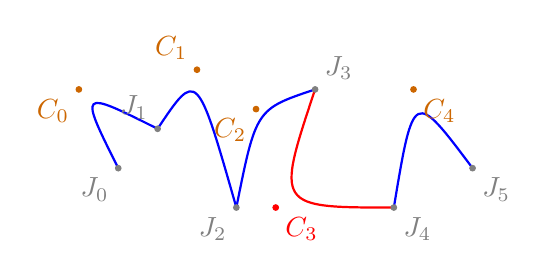
\begin{tikzpicture}[scale=0.5]
                    \coordinate (P0) at (0, 0);
                    \coordinate (P1) at (1, 1);
                    \coordinate (P2) at (3, -1);
                    \coordinate (P3) at (5, 2);
                    \coordinate (P4) at (7, -1);
                    \coordinate (P5) at (9, 0);

                    \coordinate (C0) at (-1, 2);
                    \coordinate (C1) at (2, 2.5);
                    \coordinate (C2) at (3.5, 1.5);
                    \coordinate (C3) at (4, -1);
                    \coordinate (C4) at (7.5, 2);

                    %\draw[gray, dashed] (P0) -- (P1) -- (P2) -- (P3) -- (P4) -- (P5);

                    \draw[thick, blue]   (P0) .. controls (C0) .. (P1);
                    \draw[thick, blue]   (P1) .. controls (C1) .. (P2);
                    \draw[thick, blue]   (P2) .. controls (C2) .. (P3);
                    \draw[thick, red]   (P3) .. controls (C3) .. (P4);
                    \draw[thick, blue]   (P4) .. controls (C4) .. (P5);

                    \filldraw[white!50!black] (P0) circle (2pt) node[below left] {$J_0$};
                    \filldraw[white!50!black] (P1) circle (2pt) node[above left] {$J_1$};
                    \filldraw[white!50!black] (P2) circle (2pt) node[below left] {$J_2$};
                    \filldraw[white!50!black] (P3) circle (2pt) node[above right] {$J_3$};
                    \filldraw[white!50!black] (P4) circle (2pt) node[below right] {$J_4$};
                    \filldraw[white!50!black] (P5) circle (2pt) node[below right] {$J_5$};

                    \filldraw[orange!80!black] (C0) circle (2pt) node[below left] {$C_0$};
                    \filldraw[orange!80!black] (C1) circle (2pt) node[above left] {$C_1$};
                    \filldraw[orange!80!black] (C2) circle (2pt) node[below left] {$C_2$};
                    \filldraw[red] (C3) circle (2pt) node[below right] {$C_3$};
                    \filldraw[orange!80!black] (C4) circle (2pt) node[below right] {$C_4$};

                \end{tikzpicture}
            \end{figure}
        \end{column}

    \end{columns}
        \vspace{1em}
        \item Additionally, this alleviates the issue of a high polynomial degree
    \end{itemize}
\end{frame}


\begin{frame}{B\'ezier splines: Continuity}
    \begin{itemize}
        \item In the previous example the curve is not very smooth\vspace{0.8em}
        \item To fix that, we introduce the notion of \textbf{continuity} \vspace{0.8em}
        \item B\'ezier splines can have different levels of continuity at the joint
        \vspace{0.8em}
        \begin{itemize}
            \item $C^0$-continuity refers to adjacent Bézier curves ending and starting at the same point
            \item $C^1$-continuity requires $C^0$-continuity and matching first derivative vectors at the joint
            \item $C^2$-continuity requires $C^1$-continuity and matching second derivative vectors at the joint
        \end{itemize}
        \vspace{0.8em}
        \item For \textbf{smooth curves}, $C^2$-continuity is required
    \end{itemize}
\end{frame}

\begin{frame}{B-splines}
    \begin{itemize}
        \item \strong{B-splines} (basis splines) are $C^2$-continuous B\'ezier splines \vspace{0.5em}
        \item B-splines of order $k$ are polynomial basis functions for splines of the same order, where, any spline can be represented as a linear combination of B-splines  \vspace{0.5em}
        \item Additionally, there exists a unique combination of B-splines for any given spline (de Boor, 1978) \vspace{0.5em}
        \item B-splines are fitting candidates for performing the so-called \textbf{spline interpolation} \vspace{0.2em}
        \end{itemize}
\end{frame}

\begin{frame}{B-splines: Spline interpolation}
    \begin{itemize}
        \item Spline interpolation is used to approximate functions by fitting splines, rather than using a single high-degree polynomial curve \vspace{0.2em}
        \item This process arises naturally from the formal definition of B-splines: it recursively defines each basis from a knot vector (Kaihuai, 1998),
        which indicates the positions where the splines should be connected \vspace{0.2em}
        \item Given \strong{grid G} we define a spline $S$ of $k^{\text{th}}$ order as:
            $$S_{k,G}(x) = \sum_i c_i B_{i,k}(x), \text{ where } $$
          $c_i$ are the \strong{coefficients} and $B_{i,k}(x)$ are the corresponding basis functions \vspace{0.2em}
          \begin{itemize}
            \item Liu et al. call grid what is usually called a uniform knot vector and coefficients what are usually called control points
          \end{itemize}
        \item This process maximizes pre-computed elements (\textit{minimizing possible learnable parameters})
    \end{itemize}
\end{frame}

\begin{frame}{B-splines and KANs}
    \begin{itemize}
        \item In KANs, each activation function is a $k^{\text{th}}$ order B-spline, with a $G$-valued and uniformly spaced grid  \vspace{0.3em}
        \item For each activation function what is left to learn is the coefficients of the spline \vspace{0.3em}
        \item Note that KAN also extends the grid on the edges of the spline, so that each grid point is influenced from the same number of polynomials \vspace{0.3em}
        \item Thus, for a KAN of width $W$ and depth $D$ the $\#$training parameters is $\mathbb{O}(W^2DG)$ \vspace{0.3em}
        \item The respective number of parameters for an MLP is $\mathbb{O}(W^2D)$, but KAN promises convergence with smaller widths \vspace{0.3em}
    \end{itemize}
\end{frame}

\begin{frame}{KANs: Implementation details}
    The authors used a few (questionable) tricks to train the network for optimal performance: \vspace{0.5em}
    \begin{enumerate}
        \item \textit{Residual activation functions}:
        $$\psi(x) = w_b\cdot silu(x) + w_s \cdot spline(x), \text{ where } spline(x) = \sum_i c_i B_i(x)$$
        \begin{center}
            \textit{\small \textcolor{blue!50!black}{(One can argue that this introduction of weights does not align with the initial claim)}} \vspace{1em}
        \end{center}
        \item \textit{Initialization scales}: The network's training is sensitive to initialization, so an optimal setup is introduced \vspace{1em}
    \end{enumerate}
\end{frame}

